\chapter{Downsampling circuit}

After implementing the digital filter and the Analog-Digital and Digital Analog converters, all components got integrated together in a downsampling circuit for WAV signals. The corresponding results are described in this chapter.

\section{Simple downsampling circuit}

The downsampling circuit is composed of the digital filter combined with a register, which can be found in the Verilog module \texttt{downsampling}. The task of this register is to keep only every second sample provided by the filter, in order to reduce the sampling frequency from 44.1 kHz to 22.05 kHz.\\
\\
To be able to simulate the design with WAV audio signals, additional components such as a WAV reader and a WAV writer are required. Both corresponding cell views can be found respectively in the modules \texttt{WAV\_Reader} and \texttt{WAV\_Writer}. As the read/written signals are encoded on 24 bits, as well as the filter and downsampling circuit, the connection between the 16-bit ADC and the other components is performed by a converter 24 to 16 bits (respectively 16 to 24 bits), which discards the eigth MSBs (respectively set the eight MSBs to zero). Due to the fact, that the WAV Reader and Writer only support the 16-bit WAV version, this conversion can be made without any loss of information. The corresponding modules cam be found respectively in \texttt{converterToDAC} and \texttt{converterFromADC}. 

\subsection{Simulation with sine wave signals}

For this test, the input signal is a voltage source of two added sinus waves with a DC offset of 2.5V, respective frequencies of 500 Hz and 20 kHz, and respective amplitudes of 1V and 1.5V. The corresponding schematic is provided figure \ref{fig:downsamplingSinusTestbench}. Here again, an ideal ADC is used to convert the input voltage in a digital signal. The goal of this simulation is to identify the effect of the digital filter on the input signal. Therefore, the results are stored as WAV files by means of the WAV writer, and analyzed in MATLAB. The obtained waveforms and spectrums are represented on figures \ref{fig:downsamplingSinusSignal} and \ref{fig:downsamplingSinusSpectrum}.\\
\\

\begin{figure}[!h]
	\centering 
	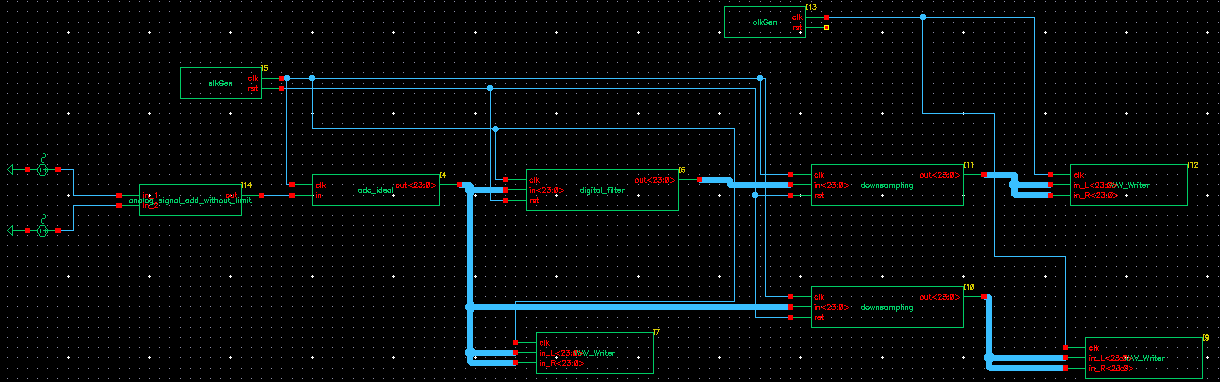
\includegraphics[scale=0.54]{images/DownsamplingCircuit/wav_downsampling_comparison.png}
	\caption{Downsampling circuit testbench (sinusoidal input voltage)}
	\label{fig:downsamplingSinusTestbench}
\end{figure} 

\begin{figure}[!h]%
	\centering
	\subfloat[Original signal]{{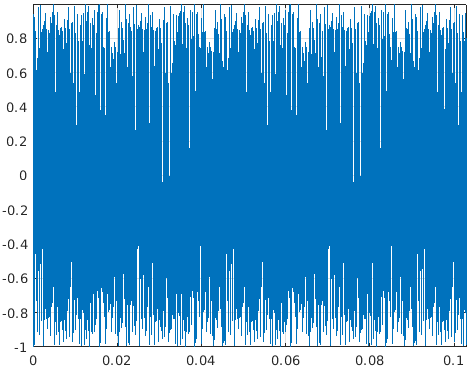
\includegraphics[scale=0.31]{images/DownsamplingCircuit/originalSignal.png}}}%
	\qquad
	\subfloat[Downsampled signal without filter]{{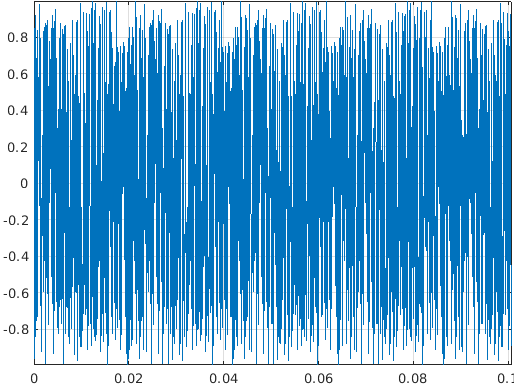
\includegraphics[scale=0.30]{images/DownsamplingCircuit/ohneFilterSignal.png}}}%
	\qquad
	\subfloat[Downsampled signal with filter]{{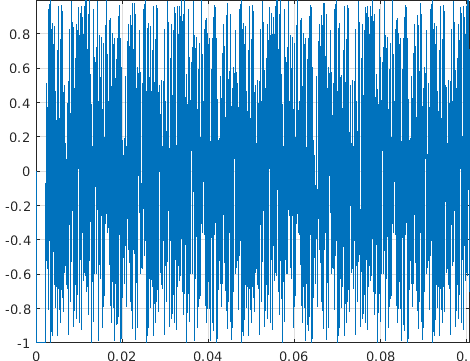
\includegraphics[scale=0.31]{images/DownsamplingCircuit/mitFilterSignal.png}}}%
	\caption{Transient simulation of the original and downsampled signals}%
	\label{fig:downsamplingSinusSignal}%
\end{figure}

\begin{figure}[!h]%
	\centering
	\subfloat[Original signal]{{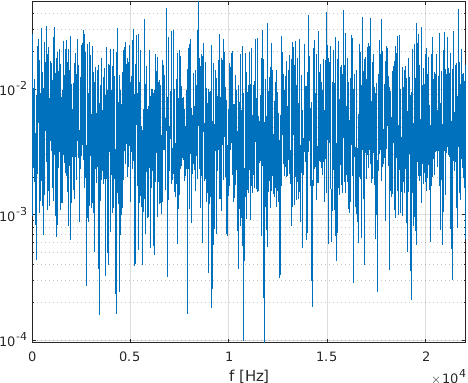
\includegraphics[scale=0.31]{images/DownsamplingCircuit/originalSpectrum.png}}}%
	\qquad
	\subfloat[Downsampled signal without filter]{{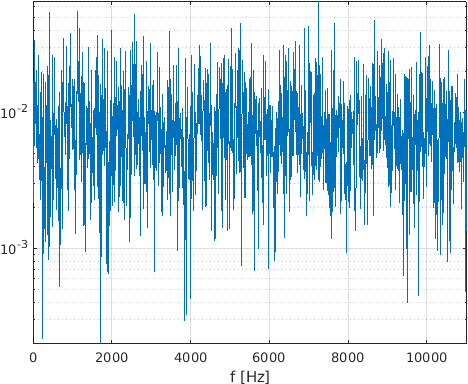
\includegraphics[scale=0.31]{images/DownsamplingCircuit/ohneFilterSpectrum.png}}}%
	\qquad
	\subfloat[Downsampled signal with filter]{{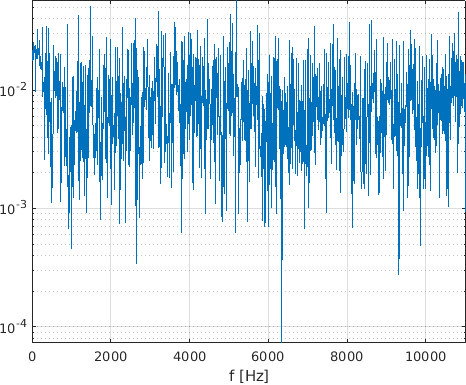
\includegraphics[scale=0.31]{images/DownsamplingCircuit/mitFilterSpectrum.png}}}%
	\caption{Spectrums (in magnitude) of the original and downsampled signals}%
	\label{fig:downsamplingSinusSpectrum}%
\end{figure}

After hearing both sampled signals, we could notice that the filtered one is a more bass sound that the other one. This confirms the fact the filter has damped the higher frequency.

%\subsection{Simulation with audio signals}

%For this test, the input signal is a stereo WAV signal, containing two channels and a wide range of harmonics. The original and the filtered/sampled signal are compared on figures ~\ref{fig:downsamplingWavEx1Signal} and ~\ref{fig:downsamplingWavEx1Spectrum} . The testbench used here is similar to the one described in the previous part.

%\begin{figure}[!h]%
%	\centering
%	\subfloat[Input signal (L and R channels)]{
%		\begin{minipage}{\linewidth}
%			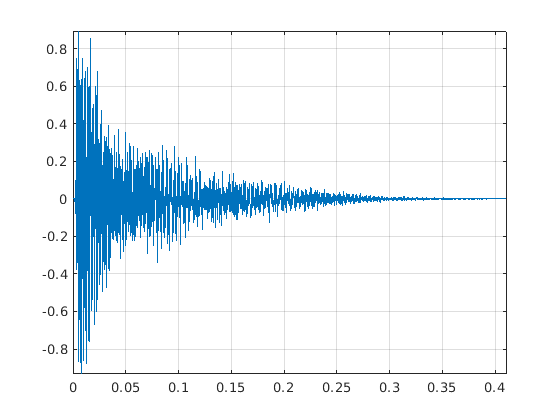
\includegraphics[scale=0.45]{images/DownsamplingCircuit/inputL.png}
%			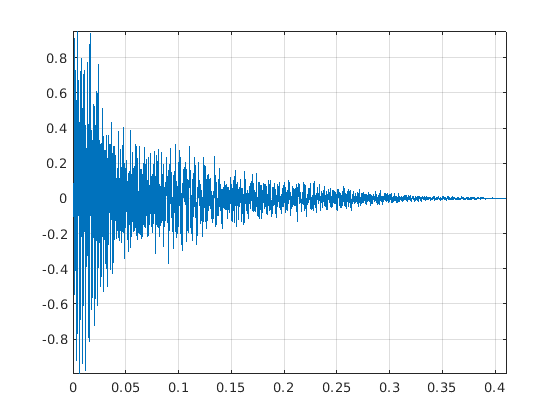
\includegraphics[scale=0.45]{images/DownsamplingCircuit/inputR.png}
%		\end{minipage}
%	}%
%	\qquad
%	\subfloat[Downsampled signal (L and R channels)]{
%		\begin{minipage}{\linewidth}
%			%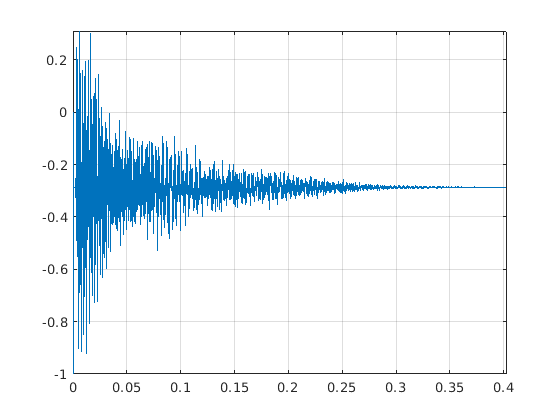
\includegraphics[scale=0.45]{images/DownsamplingCircuit/outputL.png}
%			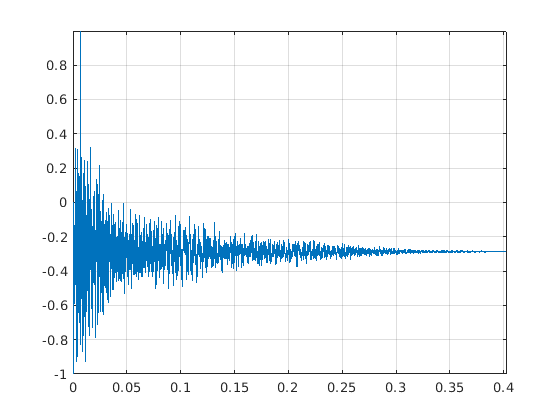
\includegraphics[scale=0.45]{images/DownsamplingCircuit/outputR.png}
%		\end{minipage}
%	}%
%	\caption{Transient waveforms of the original and downsampled signals (Example 1)}%
%	\label{fig:downsamplingWavEx1Signal}%
%\end{figure}

%\begin{figure}[!h]%
%	\centering
%	\subfloat[Input signal (L and R channels)]{
%		\begin{minipage}{\linewidth}
%			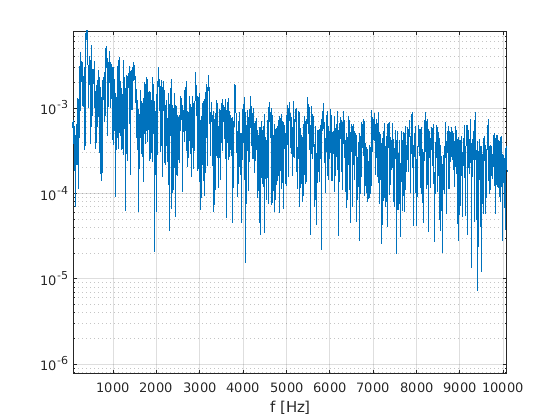
\includegraphics[scale=0.45]{images/DownsamplingCircuit/inLFFT.png}
%			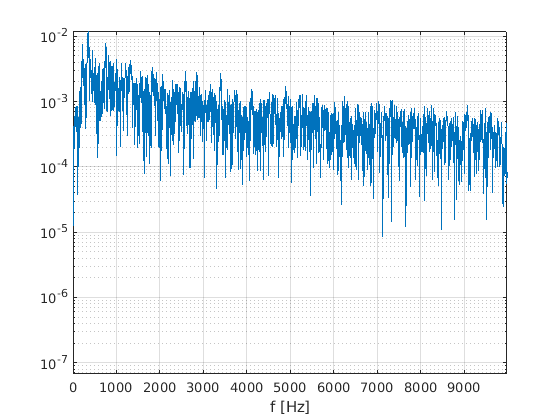
\includegraphics[scale=0.45]{images/DownsamplingCircuit/inRFFT.png}
%		\end{minipage}
%	}%
%	\qquad
%	\subfloat[Downsampled signal (L and R channels)]{
%		\begin{minipage}{\linewidth}
%			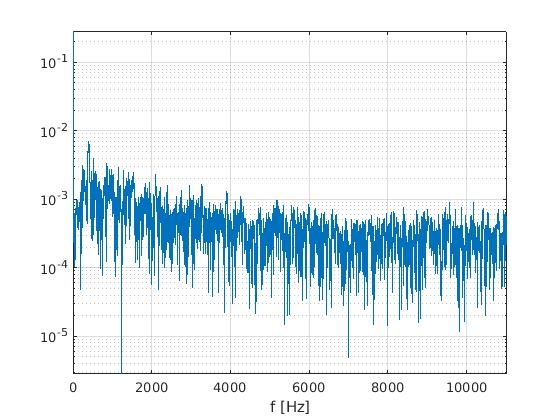
\includegraphics[scale=0.45]{images/DownsamplingCircuit/outLFFT.png}
%			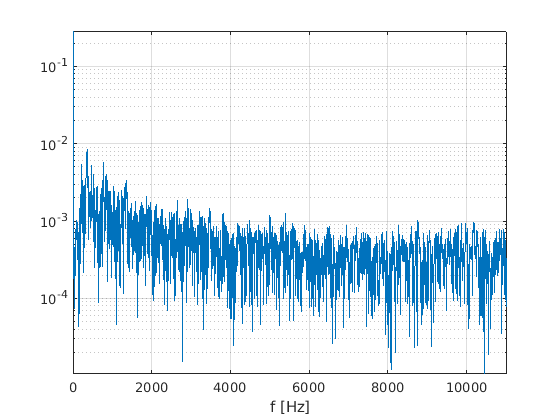
\includegraphics[scale=0.45]{images/DownsamplingCircuit/outRFFT.png}
%		\end{minipage}
%	}%
%	\caption{Spectrum (in magnitude) of the original and downsampled signals (Example 1)}%
%	\label{fig:downsamplingWavEx1Spectrum}%
%\end{figure}

%Overall, the sampled signal is quite similar to the original one, as well in terms of transient evolution as of frequency spectrums. Nevertheless, it is worth noting that the filter generates an offset of about -0.25V. This may be due to a not well fitted filter gain/coefficients, which attenuate a bit the offset component and shift the whole output signal.

%\begin{figure}[!h]%
%	\centering
%	\subfloat[Input signal (L and R channels)]{
%		\begin{minipage}{\linewidth}
%			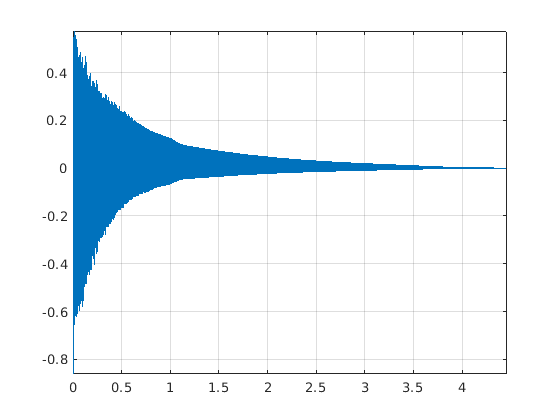
\includegraphics[scale=0.45]{images/DownsamplingCircuit/inputLEx2.png}
%			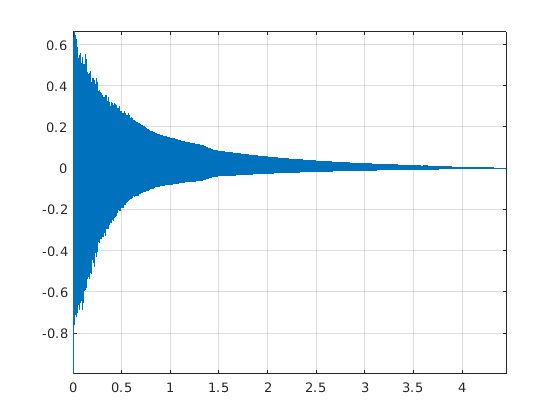
\includegraphics[scale=0.45]{images/DownsamplingCircuit/inputREx2.png}
%		\end{minipage}
%	}%
%	\qquad
%	\subfloat[Downsampled signal (L and R channels)]{
%		\begin{minipage}{\linewidth}
%			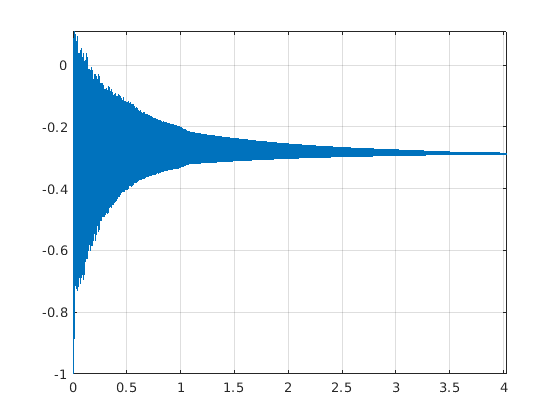
\includegraphics[scale=0.45]{images/DownsamplingCircuit/outputLEx2.png}
%			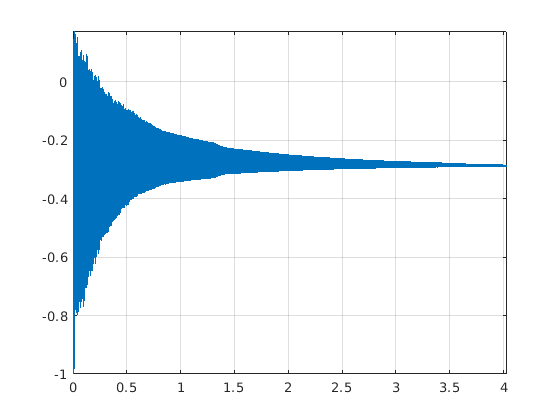
\includegraphics[scale=0.45]{images/DownsamplingCircuit/outputREx2.png}
%		\end{minipage}
%	}%
%	\caption{Transient waveforms of the original and downsampled signals}%
%	\label{fig:downsamplingWavEx2Signal}%
%\end{figure}

%\begin{figure}[!h]%
%	\centering
%	\subfloat[Input signal (L and R channels)]{
%		\begin{minipage}{\linewidth}
%			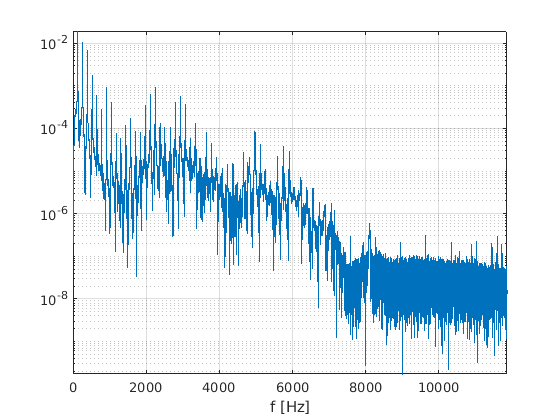
\includegraphics[scale=0.45]{images/DownsamplingCircuit/inLFFTEx2.png}
%			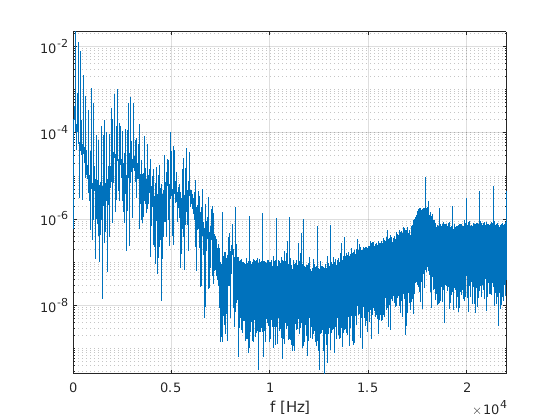
\includegraphics[scale=0.45]{images/DownsamplingCircuit/inRFFTEx2.png}
%		\end{minipage}
%	}%
%	\qquad
%	\subfloat[Downsampled signal (L and R channels)]{
%		\begin{minipage}{\linewidth}
%			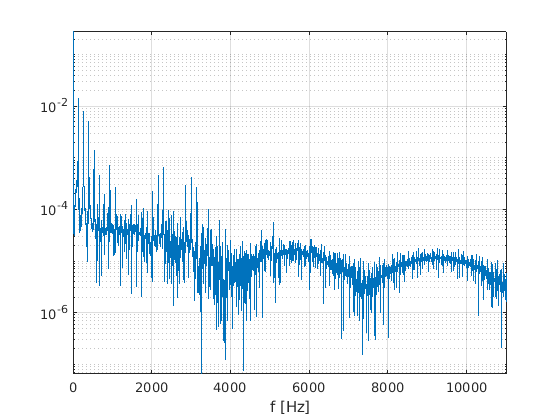
\includegraphics[scale=0.45]{images/DownsamplingCircuit/outLFFTEx2.png}
%			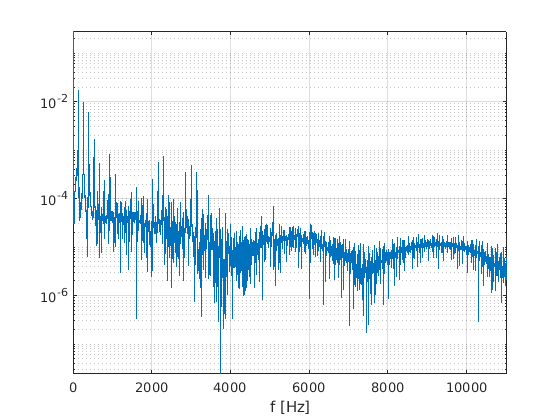
\includegraphics[scale=0.45]{images/DownsamplingCircuit/outRFFTEx2.png}
%		\end{minipage}
%	}%
%	\caption{Spectrum (in magnitude) of the original and downsampled signals (Example 2)}%
%	\label{fig:downsamplingWavEx2Spectrum}%
%\end{figure}


\section{Integration of the implemented ADC}

For this test, the ideal ADC is replaced by the extended ADC described in the second chapter. The DAC is also required to convert the digital input to an analog one for the ADC. The corresponding testbench is given in figure ~\ref{fig:downsamplingADCTestbench} The input signal is a stereo WAV signal, containing two channels and a wide range of harmonics. The original and the filtered/sampled signal are compared on figures ~\ref{fig:downsamplingWavEx1Signal} and ~\ref{fig:downsamplingWavEx1Spectrum}. 
\begin{figure}[!h]
	\centering 
	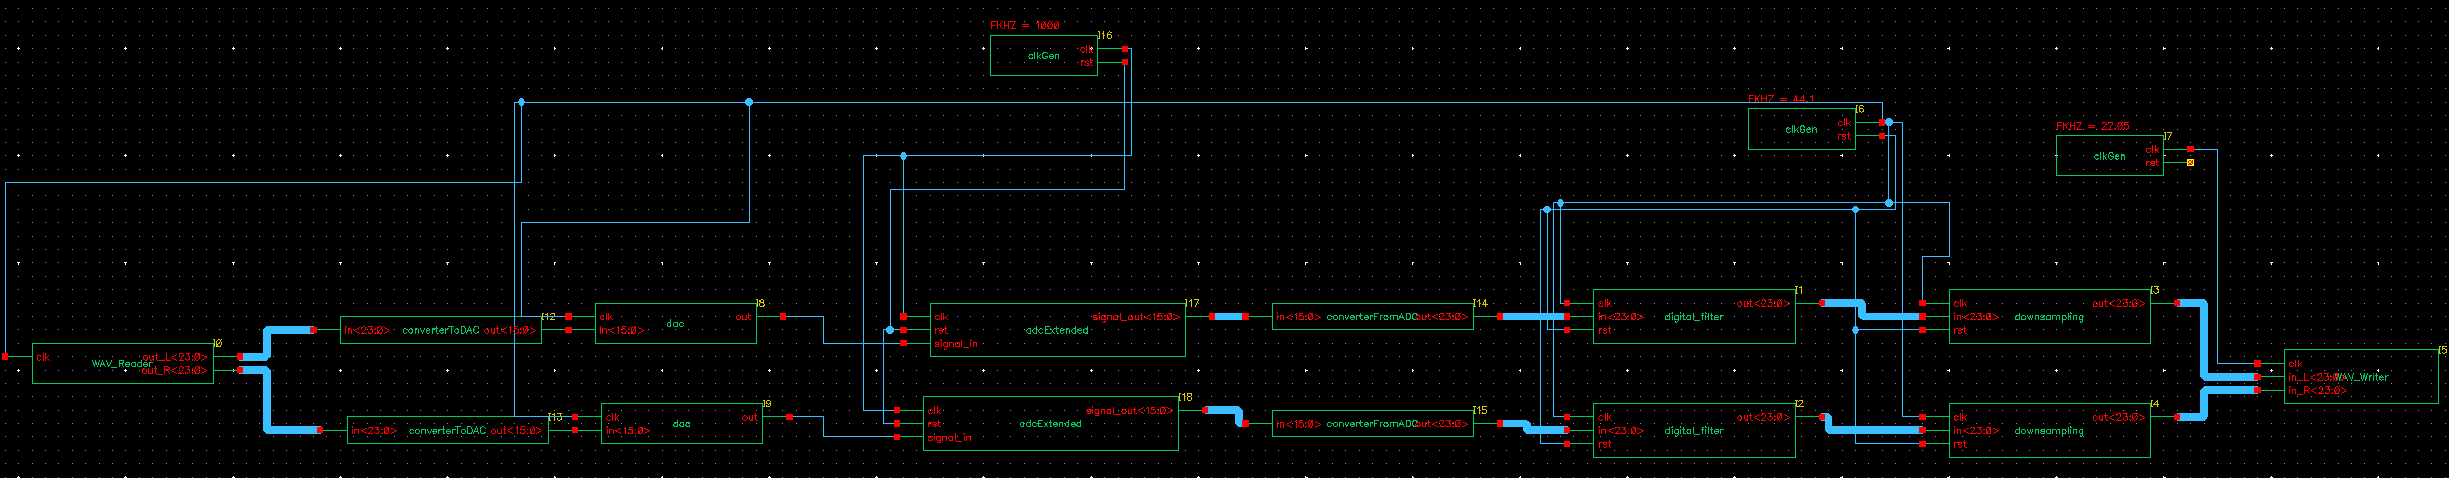
\includegraphics[scale=0.27]{images/DownsamplingCircuit/wav_downsampling.png}
	\caption{Downsampling circuit testbench (with real ADC)}
	\label{fig:downsamplingADCTestbench}
\end{figure}



\begin{figure}[!h]%
	\centering
	\subfloat[Input signal (L and R channels)]{
		\begin{minipage}{\linewidth}
			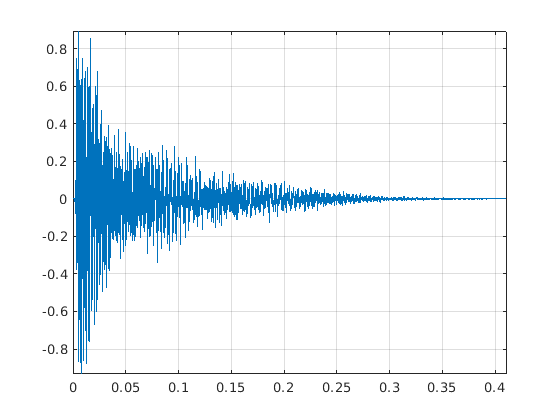
\includegraphics[scale=0.45]{images/DownsamplingCircuit/inputL.png}
			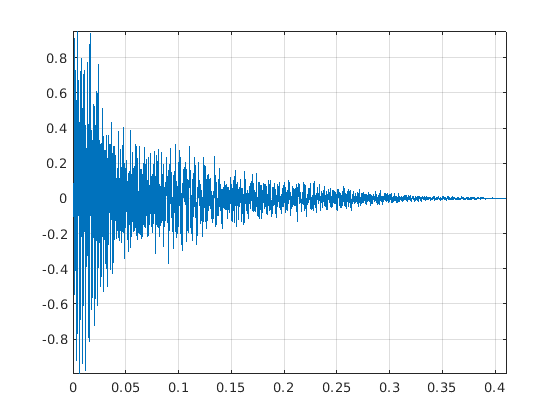
\includegraphics[scale=0.45]{images/DownsamplingCircuit/inputR.png}
		\end{minipage}
	}%
	\qquad
	\subfloat[Downsampled signal (L and R channels)]{
		\begin{minipage}{\linewidth}
			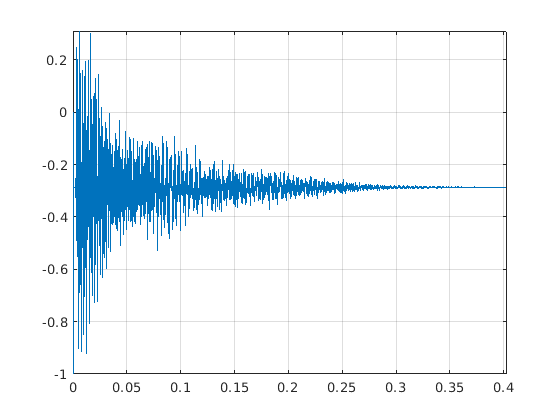
\includegraphics[scale=0.45]{images/DownsamplingCircuit/outputL.png}
			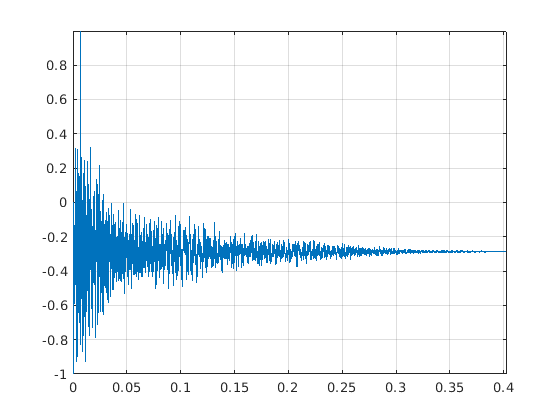
\includegraphics[scale=0.45]{images/DownsamplingCircuit/outputR.png}
		\end{minipage}
}%
	\caption{Transient waveforms of the original and downsampled signals (Example 1)}%
	\label{fig:downsamplingWavEx1Signal}%
\end{figure}

\begin{figure}[!h]%
	\centering
	\subfloat[Input signal (L and R channels)]{
		\begin{minipage}{\linewidth}
			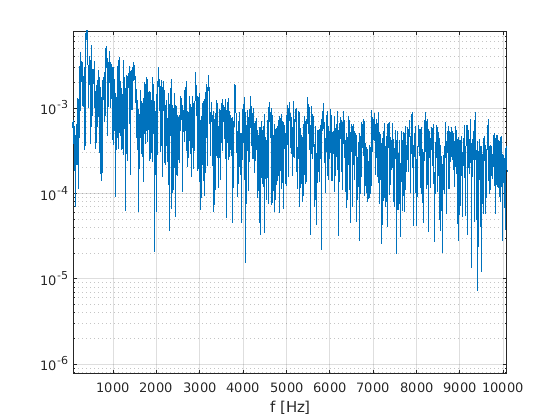
\includegraphics[scale=0.45]{images/DownsamplingCircuit/inLFFT.png}
			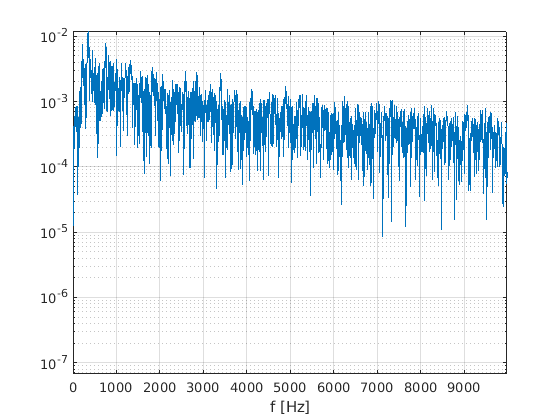
\includegraphics[scale=0.45]{images/DownsamplingCircuit/inRFFT.png}
		\end{minipage}
	}%
	\qquad
	\subfloat[Downsampled signal (L and R channels)]{
		\begin{minipage}{\linewidth}
			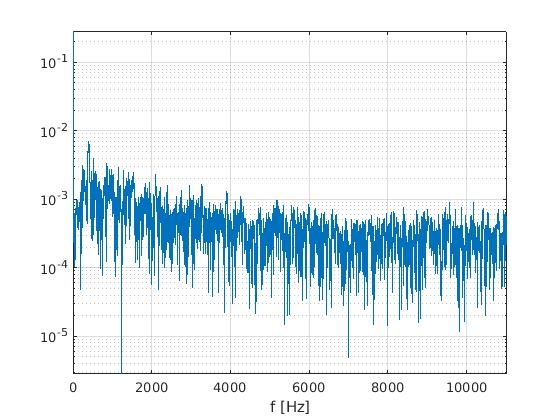
\includegraphics[scale=0.45]{images/DownsamplingCircuit/outLFFT.png}
			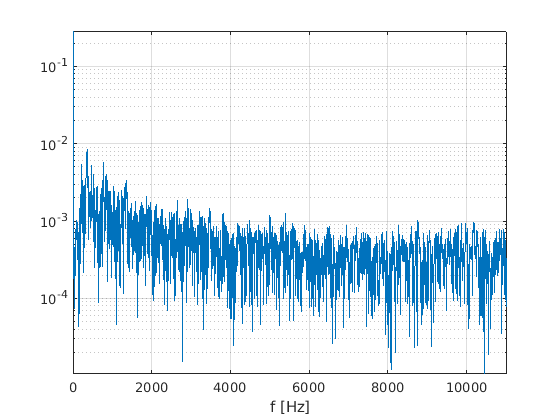
\includegraphics[scale=0.45]{images/DownsamplingCircuit/outRFFT.png}
		\end{minipage}
	}%
	\caption{Spectrum (in magnitude) of the original and downsampled signals (Example 1)}%
	\label{fig:downsamplingWavEx1Spectrum}%
\end{figure}

Overall, the sampled signal is quite similar to the original one, as well in terms of transient evolution as of frequency spectrums. The ADC does not seem to affect particularly the overall form of the input signal. Nevertheless, it is worth noting that the filter generates an offset of about -0.25V. This may be due to a not well fitted filter gain/coefficients, which attenuate a bit the offset component and shift the whole output signal. This can also be explained by the fact that the ADC tends to slightly shift the signal, because of little springs occurring at the signal extrema.